\documentclass[t]{beamer}
\usepackage{tikz}
\usepackage{pgf}
\usepackage{pgfplots}
\usetikzlibrary{positioning,shapes,shadows,arrows,calc,fadings,decorations.pathreplacing,shapes.geometric,snakes}
\usepackage{helvet}
\usepackage{calc}
\usepackage[utf8]{inputenc} % set your input encoding differently, if you want
\usepackage[english]{babel}

% Setting style of presentation
% =============================
\usetheme{NET}
\setbeamercovered{transparent=10}
\setbeamertemplate{navigation symbols}{}


% Some common packages
% ====================
\usepackage{units}
\usepackage{amsbsy}
\usepackage{amsmath}
\usepackage{amssymb}
\usepackage{graphics}
\usepackage{epsf}
\usepackage{epsfig}
\usepackage{fixmath}
\usepackage{wrapfig}
\usepackage{tikz}

\usepackage{caption}
\usepackage{subcaption}
\usepackage{float}


%\usepackage{subfigure}

\pgfrealjobname{talk}

\pgfplotsset{
	box plot/.style={
		/pgfplots/.cd,
		black,
		only marks,
		mark=-,
		mark size=\pgfkeysvalueof{/pgfplots/box plot width},
		/pgfplots/error bars/y dir=plus,
		/pgfplots/error bars/y explicit,
		/pgfplots/table/x index=\pgfkeysvalueof{/pgfplots/box plot x index},
	},
	boxb plot/.style={
		/pgfplots/.cd,
		black,
		only marks,
		mark=text,
		/pgfplots/error bars/y dir=plus,
		/pgfplots/error bars/y explicit,
		/pgfplots/table/x index=\pgfkeysvalueof{/pgfplots/box plot x index},
	},
	boxc plot/.style={
		/pgfplots/.cd,
		black,
		only marks,
		mark=x,
		/pgfplots/error bars/y dir=plus,
		/pgfplots/error bars/y explicit,
		/pgfplots/table/x index=\pgfkeysvalueof{/pgfplots/box plot x index},
	},
	box plot box/.style={
		/pgfplots/error bars/draw error bar/.code 2 args={%
			\fill[black!10,draw=black]  ##1 -- ++(\pgfkeysvalueof{/pgfplots/box plot width},0pt) |- ##2 -- ++(-\pgfkeysvalueof{/pgfplots/box plot width},0pt) |- ##1 -- cycle;
		},
		/pgfplots/table/.cd,
		y index=\pgfkeysvalueof{/pgfplots/box plot box top index},
		y error expr={
			\thisrowno{\pgfkeysvalueof{/pgfplots/box plot box bottom index}}
			- \thisrowno{\pgfkeysvalueof{/pgfplots/box plot box top index}}
		},
		 /pgf/text mark=,
		/pgfplots/boxb plot
	},
	box plot top whisker/.style={
		/pgfplots/error bars/draw error bar/.code 2 args={%
			\pgfkeysgetvalue{/pgfplots/error bars/error mark}%
			{\pgfplotserrorbarsmark}%
			\pgfkeysgetvalue{/pgfplots/error bars/error mark options}%
			{\pgfplotserrorbarsmarkopts}%
			\path ##1[dotted,line width=1pt] -- ##2;
		},
		/pgfplots/table/.cd,
		y index=\pgfkeysvalueof{/pgfplots/box plot whisker top index},
		y error expr={
			\thisrowno{\pgfkeysvalueof{/pgfplots/box plot box top index}}
			- \thisrowno{\pgfkeysvalueof{/pgfplots/box plot whisker top index}}
		},
		/pgfplots/box plot
	},
	box plot bottom whisker/.style={
		/pgfplots/error bars/draw error bar/.code 2 args={%
			\pgfkeysgetvalue{/pgfplots/error bars/error mark}%
			{\pgfplotserrorbarsmark}%
			\pgfkeysgetvalue{/pgfplots/error bars/error mark options}%
			{\pgfplotserrorbarsmarkopts}%
			\path ##1[dotted,line width=1pt] -- ##2;
		},
		/pgfplots/table/.cd,
		y index=\pgfkeysvalueof{/pgfplots/box plot whisker bottom index},
		y error expr={
			\thisrowno{\pgfkeysvalueof{/pgfplots/box plot box bottom index}}
			- \thisrowno{\pgfkeysvalueof{/pgfplots/box plot whisker bottom index}}
		},
		/pgfplots/box plot
	},
	box plot median/.style={
		/pgfplots/box plot,
		/pgfplots/table/y index=\pgfkeysvalueof{/pgfplots/box plot median index},
		TUMDarkerBlue
	},
	box plot mina/.style={
		/pgfplots/boxc plot,
		/pgfplots/table/y index=\pgfkeysvalueof{/pgfplots/box plot mina index},
		I8LogoRed,
		line width=.5pt
	},
	box plot minb/.style={
		/pgfplots/boxc plot,
		/pgfplots/table/y index=\pgfkeysvalueof{/pgfplots/box plot minb index},
		I8LogoRed,
		line width=.5pt
	},
	box plot minc/.style={
		/pgfplots/boxc plot,
		/pgfplots/table/y index=\pgfkeysvalueof{/pgfplots/box plot minc index},
		I8LogoRed,
		line width=.5pt
	},
	box plot maxa/.style={
		/pgfplots/boxc plot,
		/pgfplots/table/y index=\pgfkeysvalueof{/pgfplots/box plot maxa index},
		I8LogoRed,
		line width=.5pt
	},
	box plot maxb/.style={
		/pgfplots/boxc plot,
		/pgfplots/table/y index=\pgfkeysvalueof{/pgfplots/box plot maxb index},
		I8LogoRed,
		line width=.5pt
	},
	box plot maxc/.style={
		/pgfplots/boxc plot,
		/pgfplots/table/y index=\pgfkeysvalueof{/pgfplots/box plot maxc index},
		I8LogoRed,
		line width=.5pt
	},
	box plot width/.initial=1em,
	box plot x index/.initial=0,
	box plot median index/.initial=1,
	box plot box top index/.initial=2,
	box plot box bottom index/.initial=3,
	box plot whisker top index/.initial=4,
	box plot whisker bottom index/.initial=5,
	box plot mina index/.initial=6,
	box plot minb index/.initial=7,
	box plot minc index/.initial=8,
	box plot maxa index/.initial=9,
	box plot maxb index/.initial=10,
	box plot maxc index/.initial=1
}

\newcommand{\boxplot}[2][]{
	\addplot [box plot median,#1] table {#2};
	\addplot [forget plot, box plot top whisker,#1] table {#2};
	\addplot [forget plot, box plot bottom whisker,#1] table {#2};
	\addplot [forget plot, box plot box,#1] table {#2};
	%\addplot [forget plot, box plot mina,#1] table {#2};
	%\addplot [forget plot, box plot minb,#1] table {#2};
	%\addplot [forget plot, box plot minc,#1] table {#2};
	%\addplot [forget plot, box plot maxa,#1] table {#2};
	%\addplot [forget plot, box plot maxb,#1] table {#2};
	%\addplot [forget plot, box plot maxc,#1] table {#2};
}




% Adapt title information
% =======================
\title{An Extendable Link Layer Frame Format for Wireless Coded Mesh Networks}
\author{Martin Herrmann}
\institute{Chair for Network Architectures and Services\\ \vspace{1.5em} Department for Computer Science\\Technische Universität München}
\date{\today}





% ==============
% DOCUMENT BEGIN
% ==============
\begin{document}

% Typeset title page
% ------------------------------------------------------------------------
\setbeamertemplate{background}{\NETBlackTransparent{width=2.3\paperwidth}}
\begin{frame}
    \titlepage
\end{frame}
\setbeamertemplate{background}{}
% ------------------------------------------------------------------------


% MOTIVATION
% ------------------------------------------------------------------------
\section{Motivation a.k.a. "The Old Header"}

\begin{frame}
    \frametitle{Outline}
    \tableofcontents[currentsection]
\end{frame}

\begin{frame}
    \frametitle{Motivation a.k.a. "The Old Header"}
    \textbf{What is a Wireless (Coded) Mesh-Network?}
	
	\begin{itemize}
		\item Nodes in the network are connected wirelessly
		\item Many different possible routes $\implies $ \textbf{reliability}
		\item Combining packets using finite field arithmetic
	\end{itemize}

	\begin{figure}
	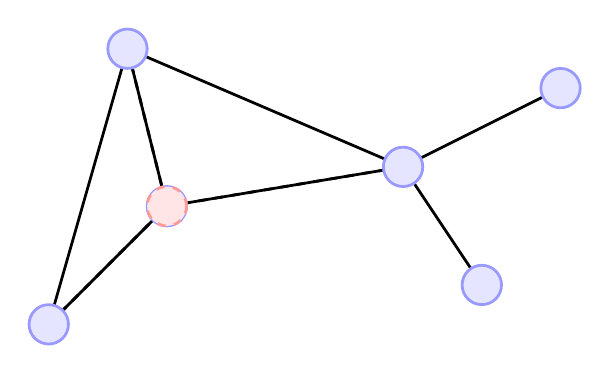
\begin{tikzpicture}[scale=.5]
		\visible<1> {
		\draw[line width=1pt] (0,0) -- (3,3);
		\draw[line width=1pt] (2,7) -- (3,3);
		\draw[line width=1pt] (9,4) -- (3,3);
		}
		\draw[line width=1pt] (9,4) -- (13,6);
		\draw[line width=1pt] (9,4) -- (11,1);

		\visible<2> {
		\draw[line width=1pt, dashed] (0,0) -- (3,3);
		\draw[line width=1pt, dashed] (2,7) -- (3,3);
		\draw[line width=1pt, dashed] (9,4) -- (3,3);
		}

		\visible<3> {
		\draw[line width=1pt] (0,0) -- (2,7);
		\draw[line width=1pt] (2,7) -- (9,4);
		}

		\draw[color=blue!40, fill=blue!10, line width=1pt] (0,0) circle(.5);
		\visible<1> {\draw[color=blue!40, fill=blue!10, line width=1pt] (3,3) circle(.5);}
		\visible<2-> {\draw[color=red!40, fill=red!10, line width=1pt, dashed] (3,3) circle(.5);}
		\draw[color=blue!40, fill=blue!10, line width=1pt] (11,1) circle(.5);
		\draw[color=blue!40, fill=blue!10, line width=1pt] (2,7) circle(.5);
		\draw[color=blue!40, fill=blue!10, line width=1pt] (9,4) circle(.5);
		\draw[color=blue!40, fill=blue!10, line width=1pt] (13,6) circle(.5);

	\end{tikzpicture}
	\end{figure}
    

\end{frame}

\begin{frame}
    \frametitle{Motivation a.k.a. "The Old Header"}
    \textbf{The old moep80211 Header}
    
    \begin{figure}
        \tikzstyle{field}=[rectangle,draw=black,line width=1pt,align=center,font=\footnotesize,minimum height=1cm]
\linespread{0.8}

\scalebox{.66}{
\begin{tikzpicture}[>=latex]
	\node[field,minimum width=2cm] at (0,0) {Frame\\Control};
	\node[field,minimum width=2cm] at (2,0) {Duration\,/\\ID};
	\node[field,minimum width=2cm] at (4,0) {MAC\,1\\(SA)};
	\node[field,minimum width=2cm] at (6,0) {MAC\,2\\(DA)};
	\node[field,minimum width=2cm] at (8,0) {MAC\,3\\(TA)};
	\node[field,minimum width=2cm] at (10,0) {SEQ};
	\node[field,minimum width=2cm] at (12,0) {MAC\,4\\(RA)};

	\node[field,minimum width=2cm,fill=black!10] at (0,-2) {Frame\\Disc.};
	\node[field,minimum width=2cm,fill=black!10] at (2,-2) {Frame\\Info};
	\node[field,minimum width=2cm,fill=black!10] at (4,-2) {Generation\\SEQ};
	\node[field,minimum width=2cm,fill=black!10] at (6,-2) {Rank Info};
	\node[field,minimum width=2cm,fill=black!10] at (8,-2) {Coefficients};
	\node[field,minimum width=2cm,fill=black!10] at (10,-2) {Ethertype};
	\node[field,minimum width=2cm,fill=black!10] at (12,-2) {Payload\\Length};

	\node[field,minimum width=4cm] at (1,-4) {Frame Body};
	\node[field,minimum width=2cm] at (4,-4) {FCS};
	
	\node[rectangle,fill=white,inner sep=0pt] at (8,-1.5) {\reflectbox{$\wr\wr$}};
	\node[rectangle,fill=white,inner sep=0pt] at (8,-2.5) {\reflectbox{$\wr\wr$}};

	\node[rectangle,fill=white,inner sep=0pt] at (1,-3.5) {\reflectbox{$\wr\wr$}};
	\node[rectangle,fill=white,inner sep=0pt] at (1,-4.5) {\reflectbox{$\wr\wr$}};

	\node[left] at (-1,1) {Octets};
	\node at (0,1) {2};
	\node at (2,1) {2};
	\node at (4,1) {6};
	\node at (6,1) {6};
	\node at (8,1) {6};
	\node at (10,1) {2};
	\node at (12,1) {6};
	
	\node[left] at (-1,-1) {Octets};
	\node at (0,-1) {2};
	\node at (2,-1) {2};
	\node at (4,-1) {2};
	\node at (6,-1) {4};
	\node at (8,-1) {2 -- 128};
	\node at (10,-1) {2};
	\node at (12,-1) {2};

	\node[left] at (-1,-3) {Octets};
	\node at (1,-3) {0 - 2162};
	\node at (4,-3) {4};

	%\draw[line width=1pt,|<->|] (14,1.2) -- +(0,-1.7);
	%\node[right,align=left] at (14.2,.35) {Generic IEEE\,802.11 header\\(30\,\unit{Byte})};
	
	%\draw[line width=1pt,|<->|] (14,-.8) -- +(0,-1.7);
	%\node[right,align=left] at (14.2,-1.65) {moep80211 header\\(16 -- 142\,\unit{Byte})};

%	\draw[line width=1pt,|<->|] (-1,-1) -- node[below] {IEEE\,802.11 MAC Header} +(14,0);

\end{tikzpicture}
}


    \end{figure}

    \begin{itemize}
        \item<2-> Very large (36 -- 172 Bytes), not all information is always of interest
        \item<3-> Different versions for different purposes, no efficient way for assembling the header
    \end{itemize}
\end{frame}
% ------------------------------------------------------------------------


% IEEE 802.11
% ------------------------------------------------------------------------
\section{IEEE 802.11}

\begin{frame}
    \frametitle{Outline}
    \tableofcontents[currentsection]
\end{frame}

\begin{frame}
    \frametitle{IEEE 802.11}
    \textbf{Why use IEEE 802.11?}

	\begin{itemize}
        \item moep80211 is based on IEEE 802.11 and cannot access the physical medium by itself \pause
        \item Advantage: can be used with existing wireless hardware \pause
        \item Disadvantage: having to "deal" with the IEEE 802.11 header
    \end{itemize}

	\pause

	\begin{figure}
		\centering
		\tikzstyle{field}=[rectangle,draw=black,line width=1pt,align=center,font=\footnotesize,minimum height=1cm]
\linespread{0.8}

\scalebox{.66}{
\begin{tikzpicture}[>=latex]
	%\draw (0,0) rectangle (2,1);
	\node[field,minimum width=2cm] at (0,0) {Frame\\Control};
	\node[field,minimum width=2cm] at (2,0) {Duration\,/\\ID};
	\node[field,minimum width=2cm] at (4,0) {MAC\,1\\(RA)};
	\node[field,minimum width=2cm] at (6,0) {MAC\,2\\(TA)};
	\node[field,minimum width=2cm] at (8,0) {MAC\,3\\(SA)};
	\node[field,minimum width=2cm] at (10,0) {SEQ};


	\node[field,minimum width=2cm] at (0,-2) {MAC\,4\\(DA)};
	\node[field,minimum width=2cm] at (2,-2) {QoS\\Control};
	\node[field,minimum width=2cm] at (4,-2) {HT\\Control};
	\node[field,minimum width=4cm] at (7,-2) {Payload};
	\node[field,minimum width=2cm] at (10,-2) {FCS};
	%\draw (2,0) rectangle (4,1);
	%\draw (4,0) rectangle (6,1);
	%\draw (6,0) rectangle (8,1);
	%\draw (8,0) rectangle (10,1);
	%\draw (10,0) rectangle (12,1);

	%\draw (0,-1.5) rectangle (2,-2.5);
	%\draw (2,-1.5) rectangle (4,-2.5);
	%\draw (4,-1.5) rectangle (6,-2.5);
	%\draw (6,-1.5) rectangle (10,-2.5);
	%\draw (10,-1.5) rectangle (12,-2.5);

	% Bits
	\node[left] at (-1,1) {Octets};
	\node at (0,1) {2};
	\node at (2,1) {2};
	\node at (4,1) {6};
	\node at (6,1) {6};
	\node at (8,1) {6};
	\node at (10,1) {2};
	
	\node[left] at (-1,-1) {Octets};
	\node at (0,-1) {6};
	\node at (2,-1) {2};
	\node at (4,-1) {4};
	\node at (7,-1) {0 -- 7951};
	\node at (10,-1) {4};
	%\draw (-1,1.5) node {\footnotesize Octets};
	%\draw (1,1.5) node {\footnotesize 2};
%	\draw (3,1.5) node {\footnotesize 2};
%	\draw (5,1.5) node {\footnotesize 6};
%	\draw (7,1.5) node {\footnotesize 6};
%	\draw (9,1.5) node {\footnotesize 6};
%	\draw (11,1.5) node {\footnotesize 2};

%	\draw (-1,-1) node {\footnotesize Octets};
%	\draw (1,-1) node {\footnotesize 6};
%	\draw (3,-1) node {\footnotesize 2};
%	\draw (5,-1) node {\footnotesize 4};
%	\draw (8,-1) node {\footnotesize 0 -- 7951 Byte};
%	\draw (11,-1) node {\footnotesize 4};
	

	% Fields
	%\draw (1,0.5) node {\footnotesize FC};
	%\draw (3,0.75) node {\footnotesize Dur};
	%\draw (3,0.25) node {\small ID};
	%\draw (5,0.5) node {\footnotesize MAC 1};
	%\draw (7,0.5) node {\footnotesize MAC 2};
	%\draw (9,0.5) node {\footnotesize MAC 3};
	%\draw (11,0.5) node {\footnotesize Seq};

	%\draw (1,-2) node {\footnotesize MAC 4};
	%\draw (3,-2) node {\footnotesize QoS};
	%\draw (5,-2) node {\footnotesize HT};
	%\draw (8,-2) node {\footnotesize Payload};
	%\draw (11,-2) node {\footnotesize FCS};
\end{tikzpicture}
}

		\caption{Generic IEEE 802.11 header}
	\end{figure}
    

\end{frame}

\begin{frame}
    \frametitle{IEEE 802.11}
    \textbf{Problems due to the IEEE 802.11 header}

	\begin{itemize}
        \item<1-> Frame format must adhere to the basic IEEE 802.11 structure
		\item<2-> A receiver must still be able to \textbf{differentiate} between moep80211 and regular frames
        \item<3-> Changing of some fields is not possible or causes problems elsewhere $\implies $ \textbf{presence of unnecessary information}
    \end{itemize}


    \begin{figure}
		\centering
		\tikzstyle{field}=[rectangle,draw=black,line width=1pt,align=center,font=\footnotesize,minimum height=1cm]
\linespread{0.8}

\scalebox{.66}{
\begin{tikzpicture}[>=latex]
	%\draw (0,0) rectangle (2,1);
	\node[field,minimum width=2cm] at (0,0) {Frame\\Control};
	\node[field,minimum width=2cm] at (2,0) {Duration\,/\\ID};
	\node[field,minimum width=2cm] at (4,0) {MAC\,1\\(RA)};
	\node[field,minimum width=2cm] at (6,0) {MAC\,2\\(TA)};
	\node[field,minimum width=2cm] at (8,0) {MAC\,3\\(SA)};
	\node[field,minimum width=2cm] at (10,0) {SEQ};


	\node[field,minimum width=2cm] at (0,-2) {MAC\,4\\(DA)};
	\node[field,minimum width=2cm] at (2,-2) {QoS\\Control};
	\node[field,minimum width=2cm] at (4,-2) {HT\\Control};
	\node[field,minimum width=4cm] at (7,-2) {Payload};
	\node[field,minimum width=2cm] at (10,-2) {FCS};
	%\draw (2,0) rectangle (4,1);
	%\draw (4,0) rectangle (6,1);
	%\draw (6,0) rectangle (8,1);
	%\draw (8,0) rectangle (10,1);
	%\draw (10,0) rectangle (12,1);

	%\draw (0,-1.5) rectangle (2,-2.5);
	%\draw (2,-1.5) rectangle (4,-2.5);
	%\draw (4,-1.5) rectangle (6,-2.5);
	%\draw (6,-1.5) rectangle (10,-2.5);
	%\draw (10,-1.5) rectangle (12,-2.5);

	% Bits
	\node[left] at (-1,1) {Octets};
	\node at (0,1) {2};
	\node at (2,1) {2};
	\node at (4,1) {6};
	\node at (6,1) {6};
	\node at (8,1) {6};
	\node at (10,1) {2};
	
	\node[left] at (-1,-1) {Octets};
	\node at (0,-1) {6};
	\node at (2,-1) {2};
	\node at (4,-1) {4};
	\node at (7,-1) {0 -- 7951};
	\node at (10,-1) {4};
	%\draw (-1,1.5) node {\footnotesize Octets};
	%\draw (1,1.5) node {\footnotesize 2};
%	\draw (3,1.5) node {\footnotesize 2};
%	\draw (5,1.5) node {\footnotesize 6};
%	\draw (7,1.5) node {\footnotesize 6};
%	\draw (9,1.5) node {\footnotesize 6};
%	\draw (11,1.5) node {\footnotesize 2};

%	\draw (-1,-1) node {\footnotesize Octets};
%	\draw (1,-1) node {\footnotesize 6};
%	\draw (3,-1) node {\footnotesize 2};
%	\draw (5,-1) node {\footnotesize 4};
%	\draw (8,-1) node {\footnotesize 0 -- 7951 Byte};
%	\draw (11,-1) node {\footnotesize 4};
	

	% Fields
	%\draw (1,0.5) node {\footnotesize FC};
	%\draw (3,0.75) node {\footnotesize Dur};
	%\draw (3,0.25) node {\small ID};
	%\draw (5,0.5) node {\footnotesize MAC 1};
	%\draw (7,0.5) node {\footnotesize MAC 2};
	%\draw (9,0.5) node {\footnotesize MAC 3};
	%\draw (11,0.5) node {\footnotesize Seq};

	%\draw (1,-2) node {\footnotesize MAC 4};
	%\draw (3,-2) node {\footnotesize QoS};
	%\draw (5,-2) node {\footnotesize HT};
	%\draw (8,-2) node {\footnotesize Payload};
	%\draw (11,-2) node {\footnotesize FCS};
\end{tikzpicture}
}

		\caption{Generic IEEE 802.11 header}
	\end{figure}

\end{frame}

% ------------------------------------------------------------------------


% A new Header Structure
% ------------------------------------------------------------------------
\section{The new Header Structure}

\begin{frame}
    \frametitle{Outline}
    \tableofcontents[currentsection]
\end{frame}

\begin{frame}
    \frametitle{The new Header Structure}
    \textbf{Basic idea}
    
   The old structure was complicated and not very efficient. Performance and expandability are improved by using following concepts: \pause
    
    \begin{itemize}
        \item Use of a \emph{generic header} that contains the basic information \pause
        \item Adding of \emph{extension headers} where special information is necessary \pause
        \item Moving the frame discriminator into the third address field of the IEEE 802.11 header
    \end{itemize}

\end{frame}

\begin{frame}
    \frametitle{The new Header Structure}
    \textbf{The new generic frame header}

    \begin{figure}
	\tikzstyle{field}=[rectangle,draw=black,line width=1pt,align=center,font=\footnotesize,minimum height=1cm]
\linespread{0.8}

\scalebox{.66}{
\begin{tikzpicture}[>=latex]
	%\draw (0,0) rectangle (2,1);
	\node[field,minimum width=2cm] at (0,0) {Frame\\Control};
	\node[field,minimum width=2cm] at (2,0) {Duration\,/\\ID};
	\node[field,minimum width=2cm] at (4,0) {MAC\,1};
	\node[field,minimum width=2cm] at (6,0) {MAC\,2};
	\node[field,minimum width=2cm,fill=gray!30] at (8,0) {Frame\\Disc};
	\node[field,minimum width=2cm] at (10,0) {SEQ};


	\node[field,minimum width=2cm] at (0,-2) {MAC\,4};
	\node[field,minimum width=2cm] at (2,-2) {QoS\\Control};
	\node[field,minimum width=2cm] at (4,-2) {HT\\Control};
	\node[field,minimum width=2cm,fill=gray!30] at (6,-2) {Next\\Header};
	\node[field,minimum width=2cm,fill=gray!30] at (8,-2) {Seq\\Number};
	\node[field,minimum width=2cm] at (10,-2) {Further\\data};

	% Bits
	\node[left] at (-1,1) {Octets};
	\node at (0,1) {2};
	\node at (2,1) {2};
	\node at (4,1) {6};
	\node at (6,1) {6};
	\node at (8,1) {6};
	\node at (10,1) {2};
	
	\node[left] at (-1,-1) {Octets};
	\node at (0,-1) {6};
	\node at (2,-1) {2};
	\node at (4,-1) {4};
	\node at (6,-1) {1};
	\node at (8,-1) {2};

\end{tikzpicture}
}

	\end{figure}
	\pause

    \textbf{Frame discriminator}
    \begin{itemize}
        \item Third address field set to value of \emph{fe:ff:ff:12:34:56} \pause
        \item Locally administered unicast MAC address \pause
        \item Should not be in regular use
    \end{itemize}

\end{frame}

\begin{frame}
    \frametitle{The new Header Structure}
    \textbf{Extension headers}

    \begin{itemize}
        \item Contain specific additional information \pause
        \item Are identified by their extension header ID (EID) in the previous header \pause
        \item Usually start with a next header field \pause
		\item May affect the data following after the extension
    \end{itemize}
    \pause

    \vspace{0.2cm}
    \begin{figure}
    \tikzstyle{field}=[rectangle,draw=black,line width=1pt,align=center,font=\footnotesize,minimum height=1cm]
\linespread{0.8}

\scalebox{.75}{
\begin{tikzpicture}[>=latex]
	%\draw (0,0) rectangle (2,1);
	\node[field,minimum width=2cm,fill=gray!30] at (0,0) {Next\\Header};
	\node[field,minimum width=4cm] at (3,0) {Extension-specific\\information};

	% Bits
	\node[left] at (-1,1) {Octets};
	\node at (0,1) {1};
\end{tikzpicture}
}

    \end{figure}

\end{frame}

\begin{frame}
    \frametitle{The new Header Structure}
    \textbf{Existing extensions}

    
    \begin{figure}
        \begin{subfigure}[b]{.45\linewidth}
        \tikzstyle{field}=[rectangle,draw=black,line width=1pt,align=center,font=\footnotesize,minimum height=1cm]
\linespread{0.8}

\scalebox{.66}{
\begin{tikzpicture}[>=latex]
	%\draw (0,0) rectangle (2,1);
	\node[field,minimum width=2cm] at (0,0) {Ethertype};
	\node[field,minimum width=2cm] at (2,0) {Payload\\length};

	%\draw (2,0) rectangle (4,1);
	%\draw (4,0) rectangle (6,1);
	%\draw (6,0) rectangle (8,1);
	%\draw (8,0) rectangle (10,1);
	%\draw (10,0) rectangle (12,1);

	%\draw (0,-1.5) rectangle (2,-2.5);
	%\draw (2,-1.5) rectangle (4,-2.5);
	%\draw (4,-1.5) rectangle (6,-2.5);
	%\draw (6,-1.5) rectangle (10,-2.5);
	%\draw (10,-1.5) rectangle (12,-2.5);

	% Bits
	\node[left] at (-1,1) {Octets};
	\node at (0,1) {2};
	\node at (2,1) {2};

	%\draw (-1,1.5) node {\footnotesize Octets};
	%\draw (1,1.5) node {\footnotesize 2};
%	\draw (3,1.5) node {\footnotesize 2};
%	\draw (5,1.5) node {\footnotesize 6};
%	\draw (7,1.5) node {\footnotesize 6};
%	\draw (9,1.5) node {\footnotesize 6};
%	\draw (11,1.5) node {\footnotesize 2};

%	\draw (-1,-1) node {\footnotesize Octets};
%	\draw (1,-1) node {\footnotesize 6};
%	\draw (3,-1) node {\footnotesize 2};
%	\draw (5,-1) node {\footnotesize 4};
%	\draw (8,-1) node {\footnotesize 0 -- 7951 Byte};
%	\draw (11,-1) node {\footnotesize 4};
	

	% Fields
	%\draw (1,0.5) node {\footnotesize FC};
	%\draw (3,0.75) node {\footnotesize Dur};
	%\draw (3,0.25) node {\small ID};
	%\draw (5,0.5) node {\footnotesize MAC 1};
	%\draw (7,0.5) node {\footnotesize MAC 2};
	%\draw (9,0.5) node {\footnotesize MAC 3};
	%\draw (11,0.5) node {\footnotesize Seq};

	%\draw (1,-2) node {\footnotesize MAC 4};
	%\draw (3,-2) node {\footnotesize QoS};
	%\draw (5,-2) node {\footnotesize HT};
	%\draw (8,-2) node {\footnotesize Payload};
	%\draw (11,-2) node {\footnotesize FCS};
\end{tikzpicture}
}

	\caption{EthertypeLength header}
	\end{subfigure}
	\begin{subfigure}[b]{.45\linewidth}
        \tikzstyle{field}=[rectangle,draw=black,line width=1pt,align=center,font=\footnotesize,minimum height=1cm]
\linespread{0.8}

\scalebox{.75}{
\begin{tikzpicture}[>=latex]
	\node[field,minimum width=2cm] at (0,0) {Padding\\(reserved)};
	\node[field,minimum width=2cm] at (2,0) {Overall\\length};

	% Bits
	\node[left] at (-1,1) {Octets};
	\node at (0,1) {2};
	\node at (2,1) {2};
\end{tikzpicture}
}

	\caption{Multipacket header}
        \end{subfigure}\\
    \vspace{0.5cm}
	\begin{subfigure}[b]{.8\linewidth}
        \tikzstyle{field}=[rectangle,draw=black,line width=1pt,align=center,font=\footnotesize,minimum height=1cm]
\linespread{0.8}

\scalebox{.66}{
\begin{tikzpicture}[>=latex]
	%\draw (0,0) rectangle (2,1);
	\node[field,minimum width=2cm] at (2,0) {Coding\\param.};
	\node[field,minimum width=2cm] at (4,0) {Generation\\SEQ};
	\node[field,minimum width=2cm] at (6,0) {Feedback};
	\node[field,minimum width=2cm] at (8,0) {Coeff.};


	\node[field,minimum width=1cm] at (0.5,-2) {Type};
	\node[field,minimum width=1cm] at (1.5,-2) {MA\\Coeff};
	\node[field,minimum width=1cm] at (2.5,-2) {SL\\Coeff};
	\node[field,minimum width=1cm] at (4,-2) {MA\\gen};
	\node[field,minimum width=1cm] at (5,-2) {RX\\rank};
	\node[field,minimum width=1cm] at (6,-2) {TX\\rank};
	\node[field,minimum width=1cm] at (7,-2) {SL\\gen};
	\node[field,minimum width=1cm] at (8,-2) {RX\\rank};
	\node[field,minimum width=1cm] at (9,-2) {TX\\rank};

	\draw[line width=1pt] (3,-0.5) -- (3,-1.5);
	\draw[line width=1pt] (1,-0.5) -- (0,-1.5);
	\draw[line width=1pt] (5,-0.5) -- (3.5,-1.5);
	\draw[line width=1pt] (7,-0.5) -- (9.5,-1.5);

	
	% Bits
	\node[left] at (0,1) {Octets};
	\node at (2,1) {2};
	\node at (4,1) {2};
	\node at (6,1) {8};
	\node at (8,1) {2 -- 128};
	
	\node[left] at (0,-3) {Bits};
	\node at (0.5,-3) {2};
	\node at (1.5,-3) {7};
	\node at (2.5,-3) {7};
	\node at (4,-3) {16};
	\node at (5,-3) {8};
	\node at (6,-3) {8};
	\node at (7,-3) {16};
	\node at (8,-3) {8};
	\node at (9,-3) {8};

\end{tikzpicture}
}

	\caption{Coding header}
        \end{subfigure}
    \end{figure}

    

\end{frame}

\begin{frame}
    \frametitle{The new Header Structure}
    \textbf{Multipacket frame format}
    \vspace{0.2cm}
    
    \begin{figure}
    \tikzstyle{field}=[rectangle,draw=black,line width=1pt,align=center,font=\footnotesize,minimum height=1cm]
\linespread{0.8}

\scalebox{.66}{
\begin{tikzpicture}[>=latex]
	%\draw (0,0) rectangle (2,1);
	\node[field,minimum width=2cm] at (-0.1,0) {Multipacket\\header};
	\node[field,minimum width=2cm] at (2,0) {EthtypeLen\\header\,1};
	\node[field,minimum width=4cm] at (5,0) {Payload\,1};

	\node[field,minimum width=6cm] at (4,-2) {. . .};

	\node[field,minimum width=2cm] at (2,-4) {EthtypeLen\\header\,$k$};
	\node[field,minimum width=4cm] at (5,-4) {Payload\,$k$};

	
	\draw [thick,decoration=brace,decorate] (7.5,0.4) -- (7.5,-4.4);
	\node at (8.5,-2) {$k$ packets};
	% Bits
	\node[left] at (-1,1) {Octets};
	\node at (0,1) {4};
	\node at (2,1) {4};
	\node at (5,1) {$n_1$};

	\node[left] at (-1,-3) {Octets};
	\node at (2,-3) {4};
	\node at (5,-3) {$n_k$};
\end{tikzpicture}
}

    \end{figure}

\end{frame}
% ------------------------------------------------------------------------


% EVALUATION
% ------------------------------------------------------------------------
\section{Evaluation}

\begin{frame}
    \frametitle{Outline}
    \tableofcontents[currentsection]
\end{frame}

\begin{frame}
    \frametitle{Evaluation}
    \textbf{Comparison of header sizes}
   
    \begin{figure}
	\setcounter{subfigure}{0}
	\begin{subfigure}[b]{.8\linewidth}
        \tikzstyle{field}=[rectangle,draw=black,line width=1pt,align=center,font=\footnotesize,minimum height=1cm]
\linespread{0.8}

\scalebox{.5}{
\begin{tikzpicture}[>=latex]
	%\draw (0,0) rectangle (2,1);
	\node[field,minimum width=6cm] at (2,0) {IEEE 802.11\\header};
	\node[field,minimum width=2cm] at (6,0) {Generic\\header};
	\node[field,minimum width=2cm] at (8,0) {Ethertype\\Length};


	\node[field,minimum width=5cm] at (1.5,-2) {IEEE 802.11\\header};
	\node[field,minimum width=2cm] at (5,-2) {Generic\\header};
	\node[field,minimum width=2cm] at (7,-2) {Ethertype\\Length};

	% Bits
	\node[left] at (-1,1) {Octets};
	\node[left] at (-1.5,0) {\bfseries Old};
	\node at (2,1) {30};
	\node at (6,1) {4};
	\node at (8,1) {4};
	\node at (12,1) {$\sum = 38$};
	
	\node[left] at (-1,-1) {Octets};
	\node[left] at (-1.5,-2) {\bfseries New};
	\node at (1.5,-1) {24};
	\node at (5,-1) {3};
	\node at (7,-1) {4};
	\node at (12,-1) {$\sum = 31$};

\end{tikzpicture}
}

		\caption{Comparison of uncoded PTM headers}
    \end{subfigure}\\
	\vspace{0.8cm}
	\begin{subfigure}[b]{.8\linewidth}
        \tikzstyle{field}=[rectangle,draw=black,line width=1pt,align=center,font=\footnotesize,minimum height=1cm]
\linespread{0.8}

\scalebox{.5}{
\begin{tikzpicture}[>=latex]
	%\draw (0,0) rectangle (2,1);
	\node[field,minimum width=6cm] at (2,0) {IEEE 802.11\\header};
	\node[field,minimum width=2cm] at (6,0) {Generic\\header};
	\node[field,minimum width=4cm] at (9,0) {Coding\\header};


	\node[field,minimum width=5cm] at (1.5,-2) {IEEE 802.11\\header};
	\node[field,minimum width=2cm] at (5,-2) {Generic\\header};
	\node[field,minimum width=4cm] at (8,-2) {Coding\\header};

	% Bits
	\node[left] at (-1,1) {Octets};
	\node[left] at (-1.5,0) {\bfseries Old};
	\node at (2,1) {30};
	\node at (6,1) {4};
	\node at (9,1) {16};
	\node at (12,1) {$\sum = 50$};
	
	\node[left] at (-1,-1) {Octets};
	\node[left] at (-1.5,-2) {\bfseries New};
	\node at (1.5,-1) {24};
	\node at (5,-1) {3};
	\node at (8,-1) {17};
	\node at (12,-1) {$\sum = 44$};

\end{tikzpicture}
}

		\caption{Comparison of coded NCM headers}
    \end{subfigure}
    \end{figure}


\end{frame}

\begin{frame}
    \frametitle{Evaluation}
    \textbf{Efficiency of header generation}

    \begin{figure}
	\setcounter{subfigure}{0}
		\centering
		\begin{subfigure}[b]{.45\linewidth}
			\scalebox{.6}{\begin{tikzpicture}

	\begin{axis} [	enlarge x limits=0.5,
					height=7cm,
					xtick=data,
					xlabel = {Implementation},
					ylabel = {Translation time [$\unit{ns}$]},
					grid=major,
					xticklabels={old,new}
		]

		\boxplot[
			forget plot,
			box plot median index=1,
			box plot whisker bottom index=2,
			box plot whisker top index=3,
			box plot box bottom index=4,
			box plot box top index=5
			%box plot mina index=6,
			%box plot minb index=7,
			%box plot minc index=8,
			%box plot maxa index=9
		] {graphics/data/translation_80211-8023.dat};
	\end{axis}

\end{tikzpicture}


}
			\caption{PTM translation times for moep80211 to IEEE 802.11}
		\end{subfigure}
		\begin{subfigure}[b]{.45\linewidth}
			\scalebox{.6}{\begin{tikzpicture}

	\begin{axis} [	enlarge x limits=0.5,
					height=7cm,
					xtick=data,
					xlabel = {Implementation},
					ylabel = {Translation time [$\unit{ns}$]},
					grid=major,
					xticklabels={old,new}
		]

		\boxplot[
			forget plot,
			box plot median index=1,
			box plot whisker bottom index=2,
			box plot whisker top index=3,
			box plot box bottom index=4,
			box plot box top index=5
			%box plot mina index=6,
			%box plot minb index=7,
			%box plot minc index=8,
			%box plot maxa index=9
		] {graphics/data/translation_8023-80211.dat};
	\end{axis}

\end{tikzpicture}


}
			\caption{PTM translation times for IEEE 802.11 to moep80211}
		\end{subfigure}
		%\caption{\small Translation times of the PTM module for moep80211 to IEEE 802.3 (left) and vice-versa (right)}
    \end{figure}

\end{frame}

\begin{frame}
    \frametitle{Evaluation}
    \textbf{Efficiency of header generation}

    \begin{figure}
		\centering
		\scalebox{.8}{\begin{tikzpicture}

	\begin{axis} [	enlarge x limits=0.25,
					height=7cm,
					width=12cm,
					xtick=data,
					xlabel = {Header building function},
					ylabel = {Translation time [$\unit{ns}$]},
					grid=major,
					xticklabels={802.11,Generic,EthertypeLength}
		]

		\boxplot[
			forget plot,
			box plot median index=1,
			box plot whisker bottom index=2,
			box plot whisker top index=3,
			box plot box bottom index=4,
			box plot box top index=5
			%box plot mina index=6,
			%box plot minb index=7,
			%box plot minc index=8,
			%box plot maxa index=9
		] {graphics/data/translation_func.dat};
	\end{axis}

\end{tikzpicture}


}
		\caption{\small Evaluation of the functions generating the different header}
    \end{figure}

\end{frame}
% ------------------------------------------------------------------------

% CONCLUSION
% ------------------------------------------------------------------------
\section{Conclusion}

\begin{frame}
    \frametitle{Outline}
    \tableofcontents[currentsection]
\end{frame}

\begin{frame}
    \frametitle{Conclusion}
    \textbf{Have the goals been reached?}

	\pause

	\begin{itemize}
		\item \textbf{Unified structure:} all frames use the same format and add extensions where needed\pause
        \item \textbf{Smaller headers:} the new structure is in many cases significantly smaller \pause
        \item \textbf{Efficency:} conversion is not significantly slower \pause
        \item \textbf{Extendability:} support of additional coding fields and new features
    \end{itemize}

\end{frame}

\begin{frame}
    \frametitle{Conclusion}
    \textbf{Future developments}

    \begin{itemize}
	
        \item moep80211 cannot be considered finished \pause
	\item Message encryption and authentication will become necessary in the future but are not supported yet\pause
        \item Addition is being developed by Julius Michaelis
    \end{itemize}
	\pause
    \begin{figure}
	\tikzstyle{field}=[rectangle,draw=black,line width=1pt,align=center,font=\footnotesize,minimum height=1cm]
\linespread{0.8}

\scalebox{.66}{
\begin{tikzpicture}[>=latex]
	%\draw (0,0) rectangle (2,1);
	\node[field,minimum width=2cm] at (0,0) {Next\\Header};
	\node[field,minimum width=2cm] at (2,0) {Info\\field};
	\node[field,minimum width=2cm] at (4,0) {Data};
	\node[field,minimum width=2cm] at (6,0) {Padding};
	\node[field,minimum width=2cm] at (8,0) {HMAC};

	\node at (5,1.8) {\footnotesize AES Encrypted};
	\draw[|<->|] (3,1.5) -- (7,1.5);

	% Bits
	\node[left] at (-1,1) {Octets};
	\node at (0,1) {1};
	\node at (2,1) {1};
	\node at (4,1) {};
	\node at (6,1) {1 -- 16};
	\node at (8,1) {20};
\end{tikzpicture}
}

	\caption{Encrypted session data format (by Julius Michaelis)}
    \end{figure}
\end{frame}
% ------------------------------------------------------------------------


\begin{frame}
    \frametitle{Bibliography}

	
        \bibliographystyle{amsalpha}
        {\footnotesize
	\bibliography{./literature.bib}}
	\nocite{*}
    

\end{frame}




\end{document}
